

%\section{System design in synthetic biology}

\section{Current understanding of the genetic toggle switch}

One of the most common devices used in synthetic biology is the genetic toggle switch. A toggle switch consists of a set of transcription factors that mutually repress each other~\autocite{Gardner:2000vha}. Genetic switches play a major role in binary cell fate decisions like stem cell differentiation, as they are capable of exhibiting bistable behaviour. Bistability of a system is defined by the existence of two distinct phenotypic states but no intermediate state. Bistability is a property that is important in nature and a valuable resource to tap into in synthetic biology. It allows cells to alter their response to environmental cues and increases the overall population fitness by 'hedge-betting' the response of the population \autocite{Veening:2008da}. 

\subsection{The genetic toggle switch in natural systems}
In developmental processes, bistability ensures that the differentiating cell will follow one pathway, or the other, with no possible intermediate phenotypes. This is vital for the correct development of a cell in a specific pathway. One example is the trophectoderm differentiation pathway, in which a mutually inhibitory toggle switch exists between Oct3/4 and Cdx2. This determines whether an Embryonic Stem cell will differentiate into a Trophectoderm cell, if Cdx2 dominates the system, or an Inner Cell Mass cell if Oct3/4 dominates~\autocite{Niwa:2005fz}. Bistability is critical in this system as a cell must differentiate into either a trophectoderm cell or an inner cell mass cell, thus the signal to do so must be straightforward. 

In the case of the GATA1 and PU.1 toggle switch, the transcription factor pair controls the fate of the common myeloid progenitors, and the two possible differentiation paths are erythroid and myeloid blood cells~\autocite{Chickarmane:2009by}. The double-negative feedback loop created by the mutually repressive pair of transcription factors sustains the system in balance until an external stimulus causes one of the two transcription factors to increase in concentration. The increased concentration of one transcription factor causes the increased repression of the production of the antagonistic transcription factor, tipping the balance towards the dominance of the first transcription factor. The double negative feedback loop reinforces this dynamic and the system remains in the same state, until an external stimulus disturbs it~\autocite{FerrellJr:2002fh}.

\subsection{Uses in synthetic biology}
Despite their simplicity, toggle switches can be powerful building blocks with which to create complex responses in a synthetic network. They can be used in isolation or in tandem to create complex networks and signalling cascades. The toggle switch has been used for the regulation of mammalian gene expression~\autocite{Deans:2007cy, Kramer:2004kq}. Other synthetic applications of the toggle switch include the construction of a synthetic genetic clock~\autocite{Atkinson:2003tu}, of a predictable genetic timer~\autocite{Ellis:2009hka}, and the formation of biofilms in response to engineered stimuli~\autocite{Kobayashi:2004cv}. 

These applications are modifications of the classical toggle switch~\autocite{Gardner:2000vha}, but an application made of a cascade or collection of the switch would be more challenging. This would make more complex applications possible and could be used to solve real-life problems. For example, an analog-to-digital converter to translate external stimuli like the concentration of an inducer into an internal digital response, or programmable bacteria to move from point to point up different chemical gradients~\autocite{Lu:2009ez}. For a review on current circuits see~\autocite{Khalil:2010hm} and for possible future applications see~\autocite{Lu:2009ez}. This leap will be difficult to achieve before first being able to build robust and well characterised individual switches.

\subsection{Modelling the genetic toggle switch} 

%Deterministic modelling utilises ordinary differential equations (ODE) and models the concentrations of the species (proteins or other molecules) by time-dependent variables~\autocite{deJong:2002ft}. When modelling deterministically the model is viewed as a system whose behaviour is entirely predictable, given sufficient knowledge. In stochastic modelling, species are measured in discrete amounts rather than concentrations and a joint probability distribution is used to express the probability that at time \textit{t} the cell contains a number of molecules of each species~\autocite{deJong:2002ft,Wilkinson:2006td}. It takes uncertainty into account and is thus often more appropriate for modelling cellular systems, although more computationally expensive. In stochastic systems the Gillespie algorithm is widely used to simulate the time-evolution of the state of the system~\autocite{Warren:2005kea}.

The toggle switch motif has been studied extensively and there are numerous studies based on a number of different methods of modelling and analysis of the dynamics, including both deterministic and stochastic approaches. The conclusions drawn about the stability and robustness of the toggle switch vary between the different modelling approaches. Numerous studies have concluded that cooperativity is a necessary condition for bistability to arise~\autocite{Gardner:2000vha, Walczak:2005ds, Warren:2004baa, Warren:2005kea, Cherry:2000wi}. However, ~\textcite{Lipshtat:2006wb} found that stochastic effects can give rise to bistability even without cooperativity in three kinds of switch; the exclusive switch, in which there can only be one repressor bound at any one time, a switch in which there is degradation of bound repressors, and the switch in which free repressor proteins can form a complex, which renders them inactive as transcription factors~\autocite{Lipshtat:2006wb}. 

In another study, \textcite{Ma:2012dt} found that the stochastic fluctuations in a system involving such a small number of molecules, like the toggle switch, uncovers effects that can not be predicted by the fully deterministic case~\autocite{Ma:2012dt}. In their system, the toggle switch was found to be tristable, as small number effects render the third unstable steady state stable. \textcite{Biancalani:2015vya} identified multiplicative noise as the source of bistability in the stochastic case~\autocite{Biancalani:2015vya}. ~\textcite{Warren:2005kea} concluded that the exclusive switch is always more robust than the general switch, since the free energy barrier is higher~\autocite{Warren:2005kea}. A summary of the toggle switch models is shown in Table~\ref{tab:refs}. As is clear from above, there is yet to exist a consensus on the stability a switch is capable of, and the most appropriate method of modelling it. Different methods arrive at different conclusions, creating confusion on which behaviour to be expected by the experimentalist for even a simple system like the toggle switch, consisting of just two genes. The toggle switch cannot be used as a building block of larger, more complex systems until its behaviour can be predicted accurately. Until then, designing systems with predictable behaviour will be near impossible.


\begin{table}[t]
\centering

\caption{Summary of stability for the CS and DP switches found via different modelling approaches}
\label{tab:refs}
\rotatebox{90}{
\begin{tabular}{@{}llll@{}}
\toprule
\multicolumn{1}{c}{} & \multicolumn{2}{c}{CS} & \multicolumn{1}{c}{DP} \\ \midrule
Stability & Deterministic & Stochastic & Deterministic \\
Monostable & \autocite{Loinger:2009vo} & \autocite{Loinger:2009vo} & \autocite{Guantes:2008gs} \\
\multirow{4}{*}{Bistable} & \autocite{Gardner:2000vha} & \autocite{Lu:2014kc}, & \multirow{4}{*}{\autocite{Guantes:2008gs}} \\
 & \autocite{Loinger:2009vo} & \autocite{Lipshtat:2006wb}, &  \\
 &  & \autocite{Biancalani:2015vya}, &  \\
 &  & \autocite{Loinger:2009vo} &  \\
\multirow{2}{*}{Tristable} & \multirow{2}{*}{} & \autocite{Loinger:2009vo}, & \autocite{Guantes:2008gs}, \\
 &  & \autocite{Ma:2012dt} & \autocite{Lu:2014kc} \\
Quadristable &  &  & \autocite{Guantes:2008gs} \\ \bottomrule
\end{tabular}
}
\end{table}

\clearpage


%\begin{table}[t]
%\centering
%\caption{Summary of stability for the CS switch found via different modelling approaches}
%\label{tab:refs}
%\begin{tabular}{@{}llll@{}}
%\toprule
%             & \multicolumn{2}{c}{CS}                                                                                                                                   & \multicolumn{1}{c}{DP}                      \\ \midrule
%Stability    & Deterministic                                      & Stochastic                                                                                          & Deterministic                               \\
%Monostable   & \autocite{Loinger:2009vo}                           & \autocite{Loinger:2009vo}                                                                            & \autocite{Guantes:2008gs}                     \\
%Bistable     & \autocite{Gardner:2000vha}, \autocite{Loinger:2009vo} & \cite{Lu:2014kc}, \autocite{Biancalani:2015vya}, \autocite{Lipshtat:2006wb}, \autocite{Loinger:2009vo} & \autocite{Guantes:2008gs}                     \\
%Tristable    &                                                    & \autocite{Loinger:2009vo}, \autocite{Ma:2012dt}                                                        & \autocite{Guantes:2008gs}, \autocite{Lu:2014kc} \\
%Quadristable &                                                    &                                                                                                     & \autocite{Guantes:2008gs}                     \\ \bottomrule
%\end{tabular}
%\end{table}

%\begin{table}[]
%\centering
%\caption{Summary of stability for the toggle switch found via different modelling approaches}
%\label{tab:refs}
%\rotatebox{90}{
%\begin{tabular}{@{}ccccccc@{}}
%\toprule
%                                        & \multicolumn{3}{c}{\textbf{Simple}}                                                                                                                                            & \multicolumn{3}{c}{\textbf{Double positive autoregulation}} \\ \midrule
%                                        & \textit{Stability}                             & \textit{Reference} & \textit{Notes}                                                                                           & \textit{Stability}  & \textit{Reference}  & \textit{Notes}  \\  \midrule
%\multirow{3}{*}{\textbf{Deterministic}} & Monostable                                     & \autocite{Loinger:2007vma}       & \begin{tabular}[c]{@{}c@{}}no cooperativity,\\ exclusive \& general\end{tabular}                         & Bistable            & \autocite{Guantes:2008gs}        &                 \\
%                                        & \multirow{2}{*}{Bistable}                      & \autocite{Gardner:2000vha}       & copperativity \textgreater 2,                                                                            & Tristable           & \autocite{Guantes:2008gs}        &                 \\
%                                        &                                                & \autocite{Loinger:2007vma}       & bound repressor degradation                                                                              & 4 steady steates    & \autocite{Guantes:2008gs}        &                 \\ \midrule
%\multirow{7}{*}{\textbf{Stochastic}}    & Monostable                                     & \autocite{Loinger:2007vma}       & \begin{tabular}[c]{@{}c@{}}no cooperativity, \\ weak repression\end{tabular}                             & Tristable           & \autocite{Lu:2014kc}             &                 \\
%                                        & \multirow{4}{*}{Bistable}                      & \autocite{Lu:2014kc}            &                                                                                                          &                     &                     &                 \\
%                                        &                                                & \autocite{Biancalani:2015vya}    & \begin{tabular}[c]{@{}c@{}}exclusive,\\ controlled by noise strength\end{tabular}                        &                     &                     &                 \\
%                                        &                                                & \autocite{Lipshtat:2006wb}      & no cooperativity                                                                                         &                     &                     &                 \\
%                                        &                                                & \autocite{Loinger:2007vma}       & \begin{tabular}[c]{@{}c@{}}no cooperativity,\\ exclusive \& \\ bound repression degradation\end{tabular} &                     &                     &                 \\
%                                        & \multicolumn{1}{l}{\multirow{2}{*}{Tristable}} & \autocite{Loinger:2007vma}       & \begin{tabular}[c]{@{}c@{}}no cooperativity,\\ strong repression\end{tabular}                            &                     &                     &                 \\
%                                        & \multicolumn{1}{l}{}                           & \autocite{Ma:2012dt}           &                                                                                                          &                     &                     &                 \\ \bottomrule 
%\end{tabular}
%}
%\end{table} 


\section{Methods in biochemical modelling}

Modelling attempts to describe the elements and dynamics of the biochemical system of interest. It is a tool used for integrating knowledge and experimental data as well as for making predictions about the behaviour of the system~\autocite{Wilkinson:2006td}. 


\subsection{Representation of transcription networks}
A transcription network can be represented in a number of ways. A network can be described by using a diagram with accompanying verbal explanations or a set of differential equations. A diagram with a lengthy verbal explanation risks the not providing sufficient clarity whereas a set of differential equations cannot easily be separated from the underlying assumptions made on the kinetics of the network. A convenient way of describing sufficient information about a system while avoiding the addition of the particular interpretation of the underlying kinetics is the use of coupled chemical reactions~\autocite{Wilkinson:2006td}. 

\subsubsection{Coupled chemical reactions and the law of mass action}

Coupled chemical reactions are often used to describe transcription networks in systems biology. They have the advantage of describing a system concisely while they can be used subsequently used for a variety of different simulation methods, each with their associated interpretation of chemical kinetics~\autocite{Wilkinson:2006td}. Coupled chemical reactions take the form


\begin{align}
	R_a + R_b \xrightarrow{k} P, \label{eq:example_eq}
\end{align}

\noindent where $R$ represents a reactant and $P$ a product. Each reaction has an associated rate $k$. A biological transcription network can be represented using the above notations. Some common examples of coupled chemical reactions used in a biological network are given in Table~\ref{tab:chem_reac_ex}. A double headed arrow represents a reversible reaction. 


\begin{table}[tb]
\centering
\caption{Examples of common genetic coupled chemical reactions. $p$ stands for promoter, and $A$ represents a protein. $A_2$ is the dimer of protein $A$.  }
\label{tab:chem_reac_ex}
\begin{tabular}{@{}ll@{}}
\toprule
Event & Coupled chemical reaction \\ \midrule
Transcription & $p  \xrightarrow{k_1} p + RNA$ \\
Dimerization & $2A \xrightleftharpoons[k_3]{k_2} A_2$ \\
Promoter repression & $A_2 + p \xrightleftharpoons[k_5]{k_4} p\bullet A_2$ \\
Activation & $A_2 + p \xrightarrow{k_6} p\bullet A_2 + RNA$ \\
Degradation & $A \xrightarrow{k_7}\oslash $ \\ \bottomrule
\end{tabular}
\end{table}

The law of mass action allows us to derive these reaction rates $k_1$-$k_7$ from the coupled chemical reactions. The assumption made in the law of mass action is that the system exists in a well mixed solution. The law of mass action states that the reaction rate is proportional to the concentration of the reactants. So for a given chemical equation as the one shown in Equation~\ref{eq:example_eq}, the rate of the reaction $k$ is defined by:
\begin{align*}
	k = [R_a][R_b]
\end{align*}



\subsubsection{Graphical representation of biochemical systems}

It is common to represent coupled biochemical reactions graphically. In a graph, as shown in Figure~\ref{fig:Toggle_switch_example}, nodes represent the species and the edges represent an interaction between the species it connects, in which a transcription factor directly affects the transcription of a gene~\autocite{Alon:2007}. An arrow at the end of an arc represents activation, i.e. that when the transcription factor binds to the promoter the rate of transcription of the gene increases. A flat line perpendicular to the arc at the end of an arc represents repression, i.e. that when the transcription factor binds to the promoter the rate of transcription of the gene decreases~\autocite{Alon:2007}.

\begin{figure}[h!]
\begin{center}
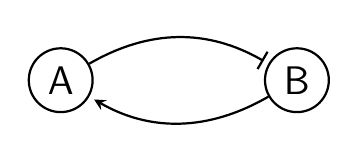
\begin{tikzpicture}	[node distance=3cm,thick,
	activate/.style={-stealth, shorten >= 2pt},
	repress/.style={-|, shorten >= 2pt},
  main node/.style={circle,fill=white,draw,font=\sffamily\Large}]

\node[main node] (1) {A};
\node[main node] (2) [right of=1] {B};
\draw[repress] [bend left] (1) to (2) {};
\draw[activate] [bend left] (2) to (1) {};
\end{tikzpicture}
\caption[A graphical representation of a biochemical system]{A graphical representation of a biochemical system. The two nodes, A and B represent species and the edges (arrows) a reaction between the two. An arrow represents activation and a flat line represents repression.}
\label{fig:Toggle_switch_example}
\end{center}

\end{figure}	



\subsubsection{\acrfull{sbml}}

The \acrfull{sbml} was developed by~\textcite{Hucka:2004wh} in order to allow for the exchange of biochemical models between software. It is an extension of the XML encoding~\autocite{DuCharme:1999} with additional fields specific to biochemical models. Software like Copasi~\autocite{Hoops:2006gy} can be used to convert a set of coupled chemical reactions to an SBML model. SBML models have been key resource for model sharing within the systems biology community~\autocite{Wilkinson:2006td} in databases like the BioModels database~\autocite{LeNovere:2006ep}. 

\subsection{Transcriptional binding kinetics}

The processes of transcription regulation in prokaryotes is complex and there have been a number of mathematical descriptions developed to approximate the dynamics observed. These include the Hill equation and the Shea-Ackers formalism. 

\subsubsection{Hill formalism}

The Hill formalism is often used to describe a biochemical system where an activator or repressor is present~\autocite{Alon:2007}. The Hill function is often represented as

\begin{align*}
	\frac{dP}{dt} = V_{max}\frac{x^n}{1 + x^n},
\end{align*}
\noindent if activation is being modelled. Parameter $n$ is the Hill coefficient and $K$ the Hill constant. $V{max}$ is the maximum amount of product and $x = \frac{S}{K}$, where S is the substrate concentration. The Hill constant represent the substrate concentration that results in half of the response and the Hill coefficient affects the steepness of the function and represents the cooperativity of the binding to the promoter~\autocite{Alon:2007}. If repression is being modelled, the Hill function is represented as

\begin{align*}
	\frac{dP}{dt} = V_{max}\frac{1}{1 + x^n}
\end{align*}



\noindent An example of the effect that the value of $n$ has on the shape of the Hill function in both activation and repression is given in Figure~\ref{fig:hill_ex}.
\newpage

\begin{figure*}[htb]
\centerfloat
    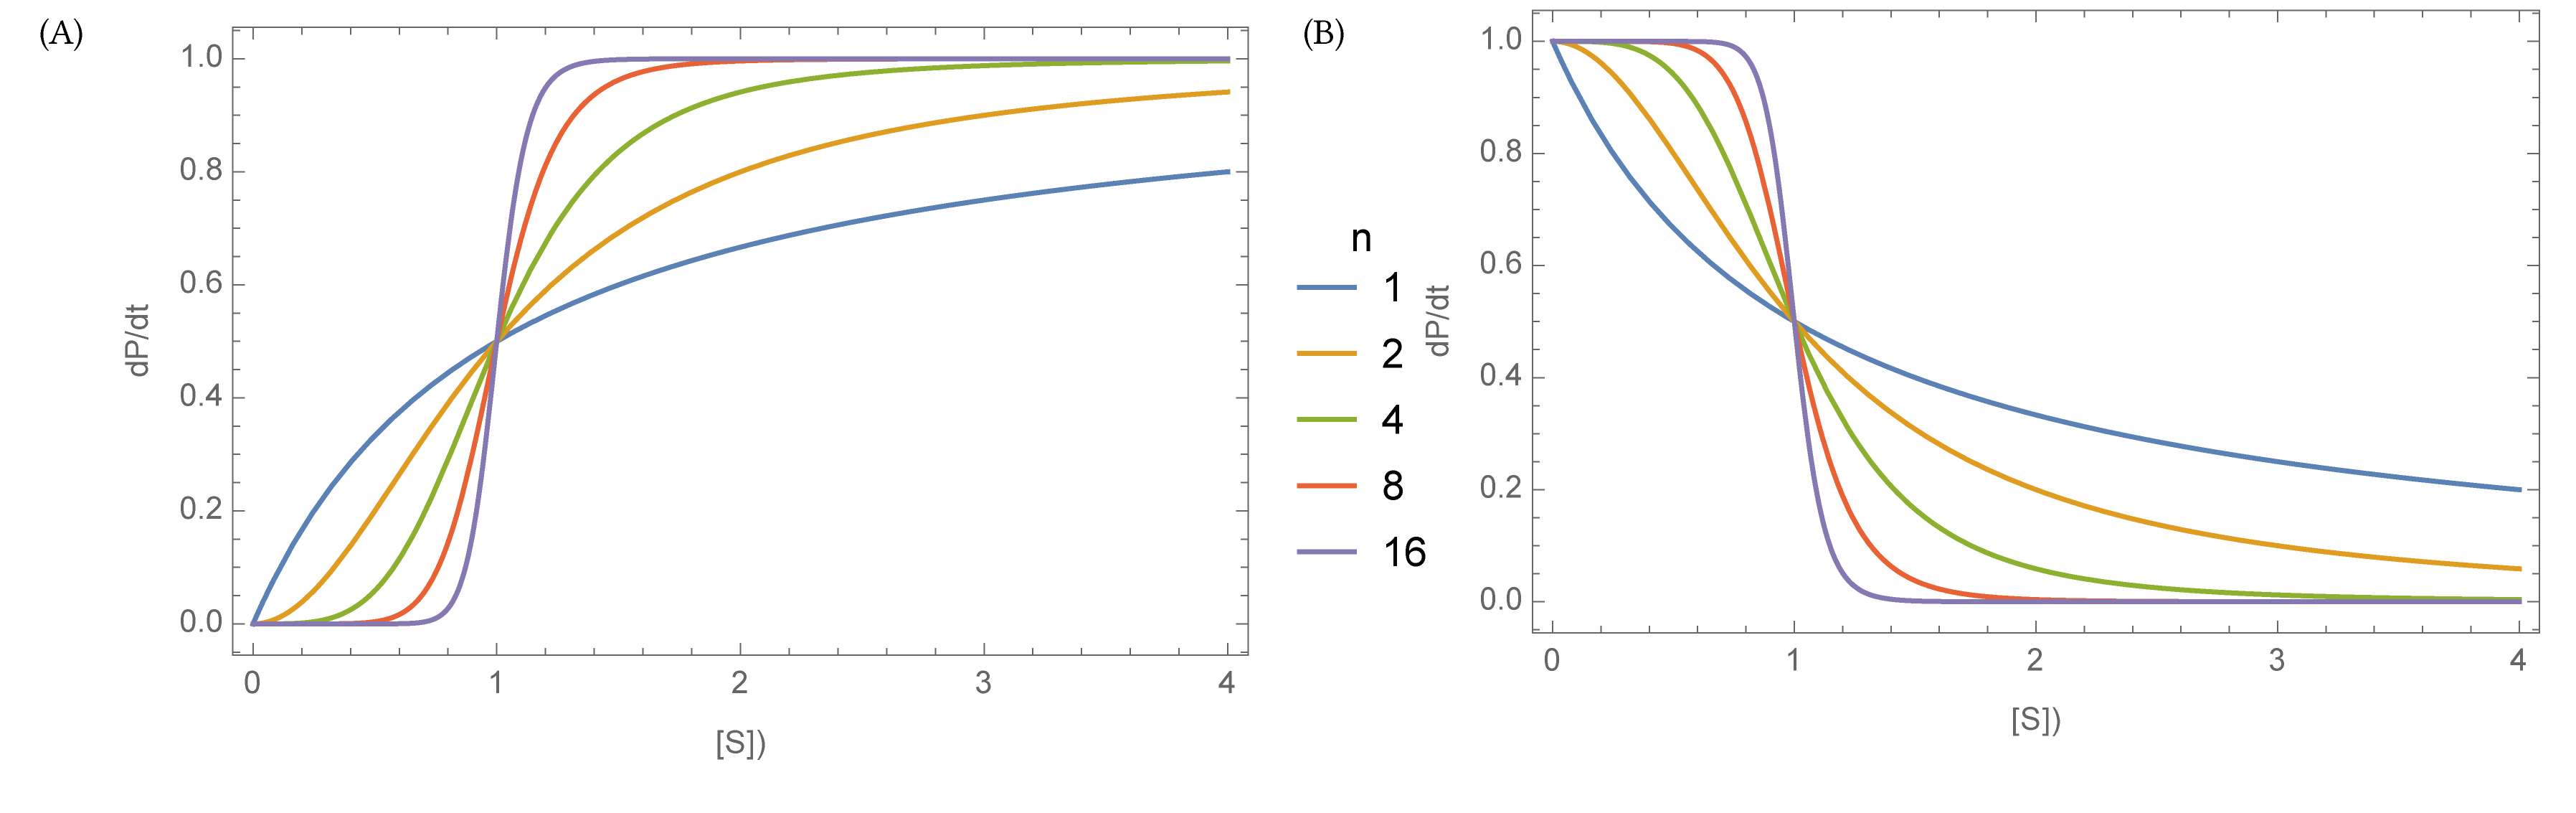
\includegraphics[scale=0.6]{../../chapters/chapterBackgr/images/hill_both-01.png}
    \caption[Hill formalism example]{The effect of different values of $n$ on the Hill function when $K$ is kept constant in the case of (A) activation and (B) repression.}
    \label{fig:hill_ex}
\end{figure*}



\subsubsection{Shea-Ackers formalism}
\label{sec:shea-ackers}
The Shea-Ackers formalism developed by~\textcite{Ackers:1982tq} uses a statistical thermodynamic model to represent the bindinf of transcription factors to their promoters. A system is described by the various states the promoter can have. An exampled of possible states is given in Figure~\ref{fig:shea_ack_ex}. Each state has an associated term, or weight, and the probability of transcription is given by the ration of the producing states over all possible states. This is referred to as the partition function. 

\begin{figure*}[htb]
\centerfloat
    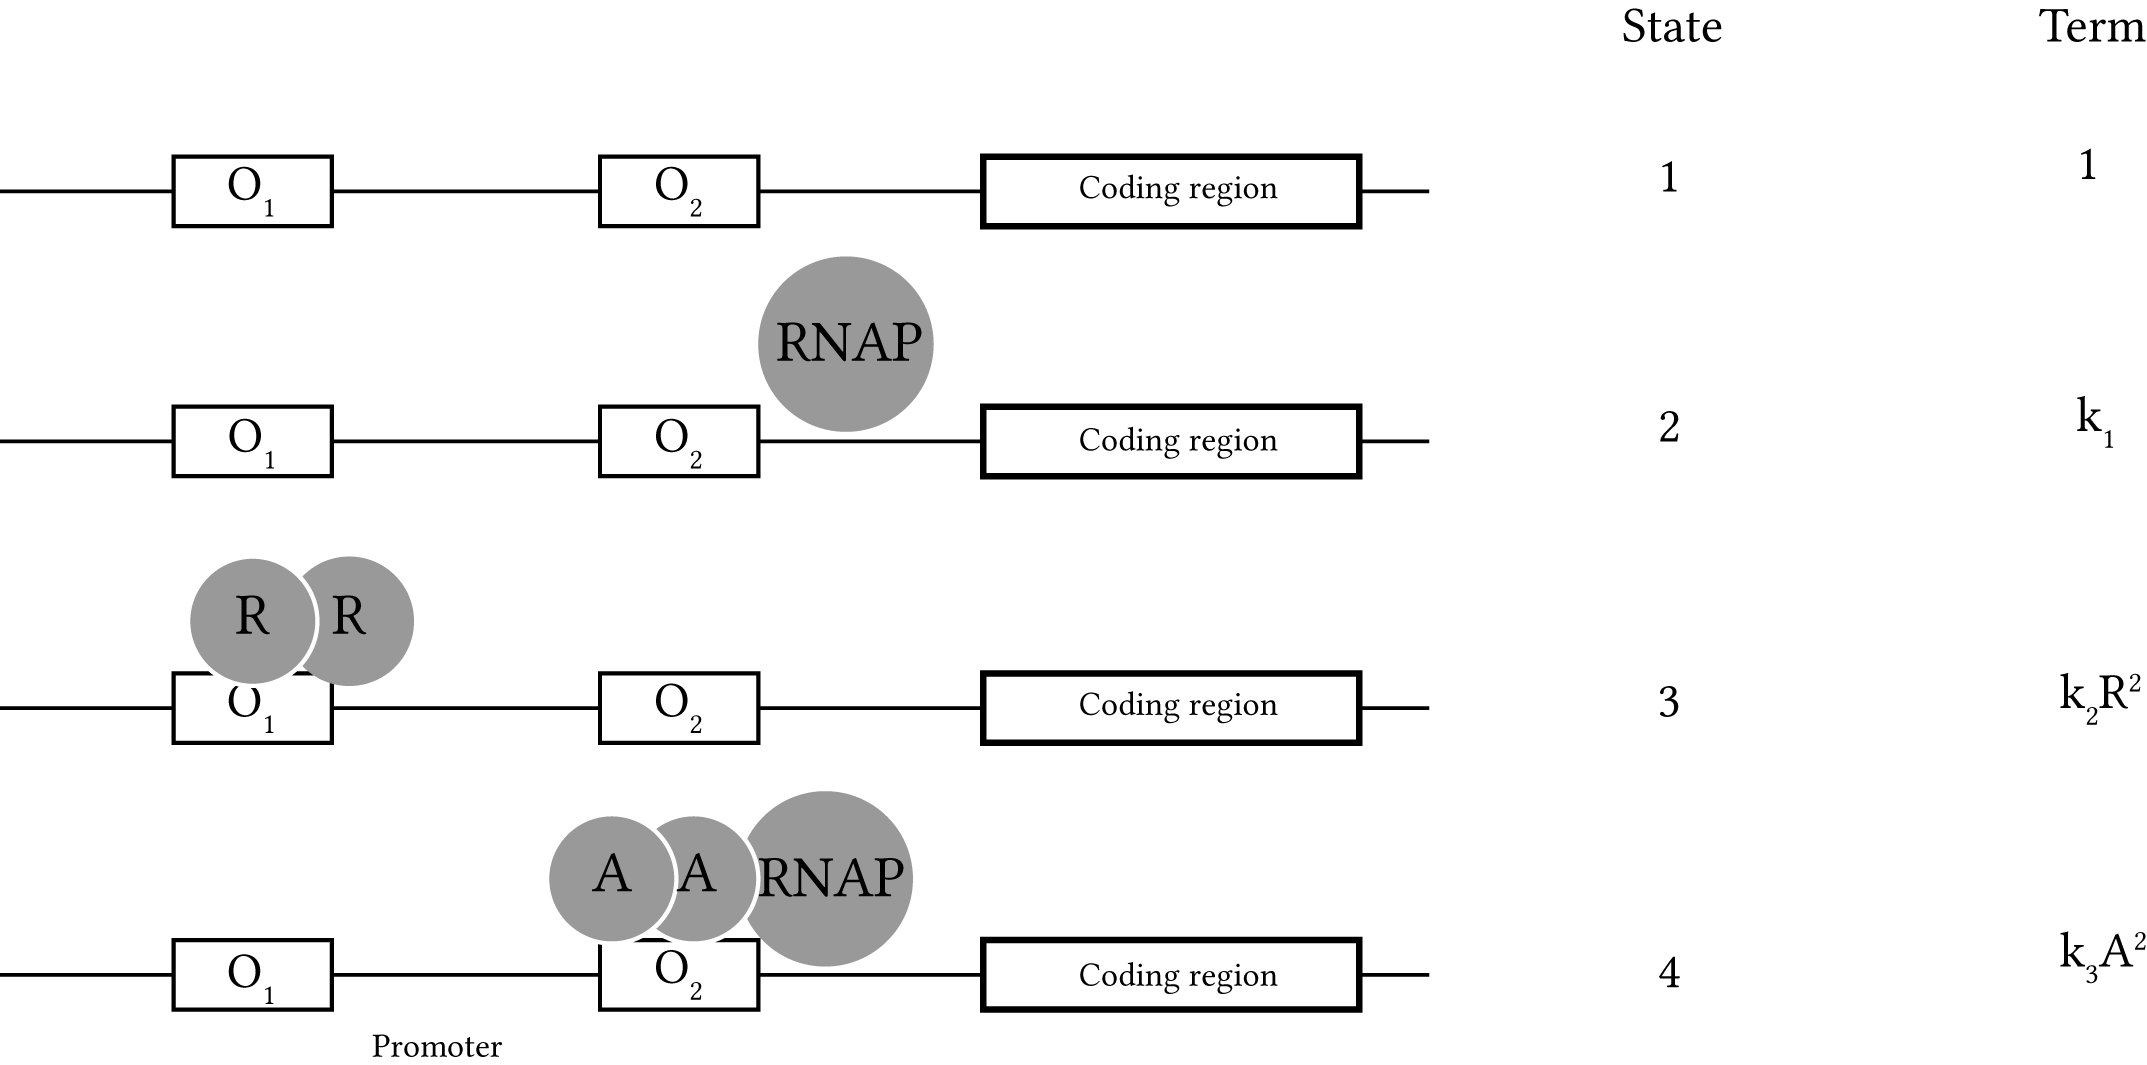
\includegraphics[scale=0.8]{../../chapters/chapterBackgr/images/shea-ackers.png}
    \caption[Shea-Ackers formalism example]{An example of a promoter regulated by a repressor (R) and an activator (A) modelled using the Shea-Ackers formalism. Figure adapted from~\textcite{Woods:2016eh}}
    \label{fig:shea_ack_ex}
\end{figure*}

The partition function is thus given by 

\begin{align}
	P_{T} = \alpha \frac{k_1 + k_{3}A^2}{1 + k_1 + k_{2}R^2 + k_{3}A^2}
\end{align}
Here I assume that repression and activation is cooperative, thus two transcription factors must bind to the promoter to repress or activate it. 
\newpage
\subsection{Simulation of dynamical systems}

There are two main ways of simulating a system, deterministically and stochastically: Deterministic modelling utilises \acrshort{ode} and models the concentrations of the species (proteins or other molecules) by time-dependent variables~\autocite{deJong:2002ft}. Rate equations are used to model gene regulation where the rate of production of a species is a function of the concentrations of the other species~\autocite{deJong:2002ft}. 

\subsubsection{Deterministic mass action kinetics}
\label{sec:predator_prey_odes}
\acrshort{ode}s are used to represent the quantitative dynamics of a biochemical network. The \acrshort{ode}s describing a system can be derived from the coupled chemical reactions descibing the system as well as their associated rates. This will be illustrated using a simple example, the Lotka-Voltera predator-prey model~\autocite{lotka:voltera}. This system describes the dynamics between two interacting species, a predator and a prey. The chemical reactions describing the system are given in Table~\ref{tab:pp_reac}. The rates of the system are organised to vector form:


\begin{table}[h]
\centering
\caption{Predator-prey chemical reactions}
\label{tab:pp_reac}
\begin{tabular}{@{}lll@{}}
\toprule
Name & Reaction & Rate \\ \midrule
prey birth & $x \xrightarrow{k_1} 2x$ & $k_{1}x$ \\
predation & $x + y \xrightarrow{k_2} 2y$ & $k_{2}xy$ \\
predator death & $y \xrightarrow{k_3} \oslash$ & $k_{3}y$ \\ \bottomrule
\end{tabular}
\end{table}

\begin{align*}
h = 
\begin{pmatrix}
	k_{1}x \\
	 k_{2}xy \\
	 k_{3}y 
\end{pmatrix}
\end{align*}
The stoichiometry matrix of the system is $m\times n$ matrix, where $m$ is the number of species and $n$ the number of reactions and it summarises the stoichiometries of the system.  
\begin{align}
S = \begin{pmatrix}
	1 & -1& 0\\
	0&1&-1 
\end{pmatrix}
\end{align}
The \acrshort{ode}s can then be constructed by multiplying the stoichiometry matrix $S$ by the matrix containing the rates $h$. Therefore
\begin{align}
s(t) = \frac{d}{dt}\begin{pmatrix}
x\\
y 
\end{pmatrix} = \begin{pmatrix}
1 &-1  &0 \\ 
 0&1  &-1 
\end{pmatrix}\begin{pmatrix}
k_1[x]\\
k_2[x][y]\\
k_3[y] 
\end{pmatrix}
\end{align}
and thus we get the two \acrshort{ode}s describing the system as

\begin{align}
\frac{dx}{dt} &= k_1x - k_2xy\\ \label{eq:predator-prey}
\frac{dy}{dt} &= k_2xy - k_3y
\end{align}

\noindent These differential equations can be simulated numerically over time using software packages like Mathematica~\autocite{mathematica:2016} and Python.

\subsubsection{Assumptions of deterministic modelling}

Two key assumptions are made when modelling a biochemical system using \acrshort{ode}s. Firstly, the species present in the system are measured continuously rather than discreetly. This means that the species are measured in concentration over time and not number of molecules over time. This assumption requires at least 1000 molecules to be present in order to be met~\autocite{iglesias:2010}. The second assumption made is that the reactants are in a well mixed solution. This means that the species in the system can interact each other constantly and freely. 


\subsection{Nonlinear dynamical modelling}

\subsubsection{Phase plane analysis}
An alternative to studying the trajectory of a dynamical system over time is to study its behaviour in the phase plane. During a phase plane analysis the dependent variables $x$ and $y$ are plotted against eachother, as shown in Figure~\ref{fig:pp_phase}.

\begin{figure*}[htb]
\centerfloat
    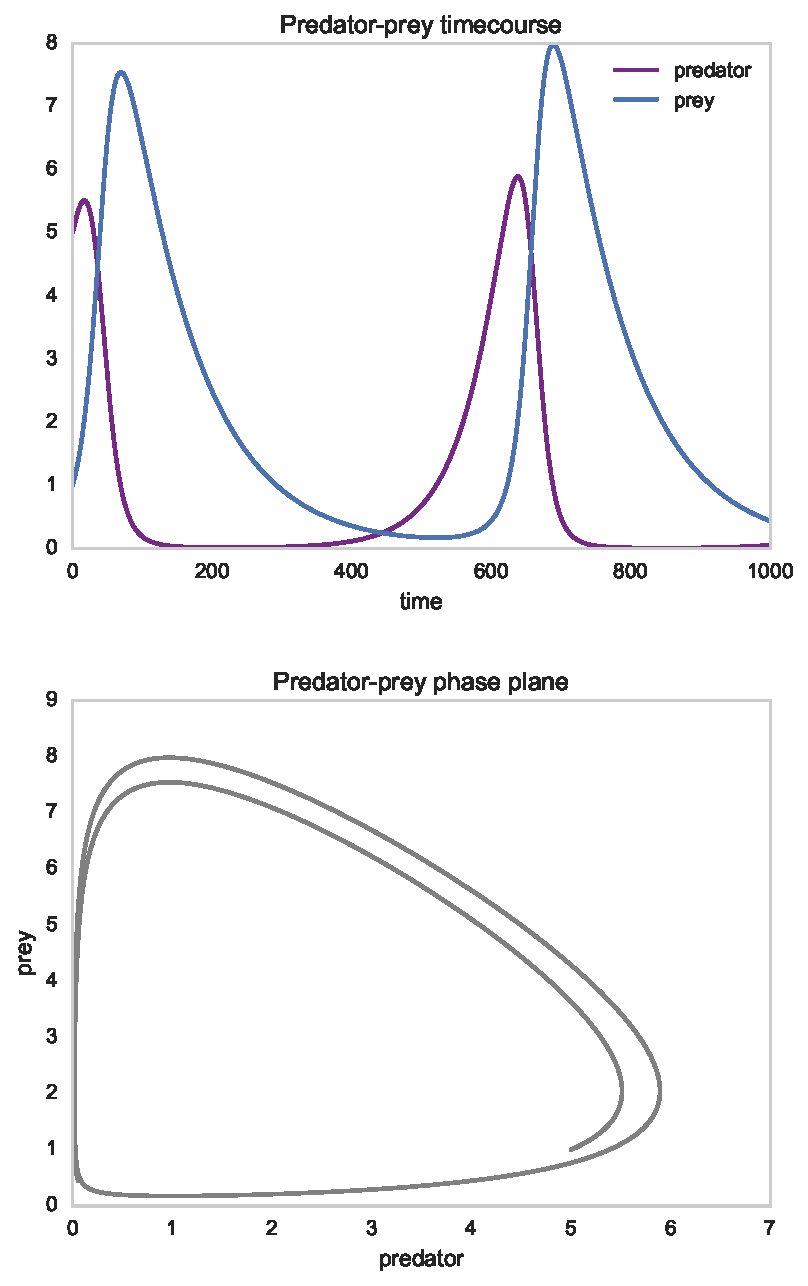
\includegraphics[scale=0.7]{../../chapters/chapterBackgr/images/pp-phaseplane.pdf}
    \caption[Phase plane analysis]{(A) The predator-prey system of equations as defined in Section~\ref{sec:predator_prey_odes} trajectory over time (B) Phase plane plot of the predator-prey system of equations. The parameters used here are $k_1=2$, $k_2=1$ and $k_3=1$.}
    \label{fig:pp_phase}
\end{figure*}

\subsubsection{Steady states}

For a system $s$, any system satisfying $\frac{d}{dt}s(t) = 0$ is considered a fixed point, or steady state. At that point the dynamics of the system are considered in equilibrium and will not change with increasing time. Using the example of the predator-prey system, a steady state exists when the system of Equations~\ref{eq:predator-prey} are equal to 0: 
 
\begin{align}
\frac{dx}{dt} &= f_x(x,y) = k_{1}x - k_{2}xy = 0\\
\frac{dy}{dt} &= f_y(x,y) = k_{2}xy - k_{3}y = 0
\end{align}

By solving this system of equations, we get two steady states. One when $x = y = 0$ and one when $x = \frac{k_3}{k_2}$ and $y = \frac{k_1}{k_2}$. The stability of each steady state can then be determined.

\subsubsection{Steady state stability} 

A stable steady state is defined as a fixed point whose nearby points approach the fixed point~\autocite{kaplan:1959}. This means that after a small perturbation the system will quickly return to the steady state. An unstable steady state is one which if the system is perturbed slightly then it moves away from the steady state~\autocite{konopka:2007}. The stability of the fixed points can be determined by the sign of the eigenvalues of the Jacobian matrix at each point. The Jacobian matrix is given by 

\begin{align}
\textbf{J} = \begin{pmatrix}
	\frac{\partial f_x}{\partial x} & \frac{\partial f_x}{\partial y}\\
	\frac{\partial f_y}{\partial x} & \frac{\partial f_y}{\partial y}	
\end{pmatrix}
\end{align}


\noindent Using the predator-prey system as an example, the Jacobian matrix is given by

\begin{align}
\textbf{J} = \begin{pmatrix}
	k_1 - k_{2}y & -k_{2}x\\
	k_{2}y & k_{2}x - k_3 
\end{pmatrix}
\end{align}

\noindent The eigenvalues λ are given by

\begin{align}
\det(\mathbf{J} - λ\mathbf{I})
\end{align}

\noindent where det is the determinant and \textbf{I} the identity matrix. If both eigenvalues are real and negative or imaginary with a negative real part then the steady state is stable. If both eigenvalues have a positive real part then the steady state is unstable and if one has a positive and one has a negative fixed part the steady state is an unstable saddle node. If both eigenvalues are purely imaginary, the system oscillates around the fixed point. Solving the above for the fixed points in the predator-prey system, we find one stable steady state and one oscillatory fixed point. 

\subsection{Stochastic modelling of dynamical systems}

The assumptions that have to be made to model a system deterministically cannot always be met. This can occur when the molecule numbers in the system are low or the solution cannot be assumed to be well mixed. When this is the case, stochastic dynamics are more appropriate to model dynamical system. In stochastic modelling species are measured in discrete amounts rather than concentrations and a joint probability distribution is used to express the probability that at time \textit{t} the cell contains a number of molecules of each species~\autocite{deJong:2002ft,khamash_iglesias:2010}. It takes uncertainty into account and does not assume a well mixed solution. 

Biological processes are well known to include randomness. The source of this randomness originates from the random collisions between molecules that govern biological reactions~\autocite{khamash_iglesias:2010}. This randomness affects downstream events and affect the phenotypic behaviour of cells. This is known as cellular noise and it is known to be key for various cellular processes~\autocite{Eldar:2010kk}. Cellular noise can be classified into two categories, intrinsic noise and extrinsic noise. Intrinsic noise originates from the inherently random collisions between the species of the system under consideration. Extrinsic noise originates from fluctuations in the environment within which the system of interest resides, like the number of available RNA polymerases or other protein numbers~\autocite{khamash_iglesias:2010}. The noisiness of biological processes often make stochastic dynamics more appropriate for modelling cellular systems.  


%Stochastic modelling is used to describe systems that behave discretely and stochastically~\autocite{Wilkinson:2006td}. It takes into account the randomness in the behaviour of the species involved in a biochemical system, known as 'intrinsic' noise. The probability that a given species will have a certain number of molecules at time t is described by a stochastic simulation~\autocite{khamash_iglesias:2010}.   

\subsubsection{Simulating stochastic models}

Stochastic models are often analytically intractable but can be studied using numerical simulation. A well known algorithm for the simulation of such models is the Direct method proposed by~\textcite{Gillespie:1977ww}.

%Stochastic models can be simulated using a number of different methods. Here I will describe the use of Monte Carlo simulations, as these are used throughout this thesis. The most widely used of the Monte Carlo algorithms is the Gillespie algorithm, described below. 


\subsubsection{The Gillespie algorithm}
 In stochastic systems the Gillespie algorithm is widely used to simulate the time-evolution of the state of the system~\autocite{Wilkinson:2006td}. The algorithm, developed by~\textcite{Gillespie:1977ww} can be summarised in four steps:
%What type of random numbers are generated for each of these? How does the time-step one work? (i.e. is there a limit on the length of timestep that can be produced?)
\begin{enumerate}
\item Initialise time $t$ and number of species $s$ and state of system $x$
\item Draw a sample timestep τ from the distribution of time $Τ$
\item Draw a sample reaction from all reactions $R$
\item Update time by $t = t + τ$ and state of system by $x = x + s_μ$
\item Repeat from Step 2 until total simulation time reached
\end{enumerate}
   
\noindent This algorithm results in one trajectory of the system. It has to be repeated a number of times to obtain enough realisations of the trajectory to compute appropriate summary statistics.

\subsubsection{Stochastic mass action kinetics}
Here I will consider the predator-prey system introduced in Section~\ref{sec:predator_prey_odes}. A set of reactions is defined, as shown in Table~\ref{tab:pp_reac}, and each one has an associated stochastic rate constant $c_i$. The rate constant, or hazard function, of each reaction i is defined as $h_i(x, c_i)$, where x is the current state of each species in the system.The form of each hazard function is defined by the order of the given reaction~\autocite{Wilkinson:2006td}, as shown in Table~\ref{tab:hazards}. 


\begin{table}[h]
\centering
\caption{Defining reaction hazards}
\label{tab:hazards}
\begin{tabular}{@{}lll@{}}
\toprule
Order & Reaction & Hazard \\ \midrule
Zeroth & $\oslash \xrightarrow{c_i}X $ & $h_i(x, c_i) = c_i$ \\
First & $X_j \xrightarrow{c_i} ? $ & $h_i(x, c_i) = c_{i}x_j$ \\
Second & $X_j + X_k \xrightarrow{c_i} ? $ & $h_i(x, c_i) = c_{i}x_{j}x_k$ \\
Dimerization & $X_j + X_j \xrightarrow{c_i} X_{2j} $ & $h_i(x, c_i) = c_{i}\frac{x_{j}(x_{j}-1)}{2}$ \\ \bottomrule
\end{tabular}
\end{table}

\noindent Therefore, when simulating a stochastic system using the Gillespie algorithm, the state of the system $x$ is defined as the sum of all the reaction hazards, namely $h_0(x, c) = \sum_{i=1}^{n}h_{i}(x, c_i)$~\autocite{Wilkinson:2006td}. 

\section{The Bayesian solution to parameter inference and system design}

%For a model to be used in a systems biology setting the parameters must first be defined. 
The parameters of a model represent the biochemical rates that are involved in the system under study, like degradation rates, transcription rates and polymerization rates. These rates cannot always be measured experimentally and taking generalised estimates from existing literature can be inaccurate. In order to make useful predictions about the biological system under consideration, the model parameters must be estimated~\autocite{Zheng:2010bp}. 

To address this challenge, statistical optimization methods have been developed. These methods aim to infer the parameters of the model that can give rise to some experimentally observed behaviour. Parameter inference methods have the same general structure: there is a cost function that compares the model data to the experimental data and an optimization function that aims to optimize the cost function~\autocite{Toni:2010}. There is a wide range of such optimization algorithms that can be used like gradient decent~\autocite{Levenberg:1944we, Marquardt:1963wr}, simulated annealing~\autocite{Kirkpatrick:1983kv} and evolutionary algorithms~\autocite{Onbasoglu:2001um, Wood:2002uo}.  

Bayesian approaches to parameter inference have been shown to work well in biological problems~\autocite{Barnes:2011hh, Toni:2010, Liepe:2014iw}. Bayesian approaches to parameter inference have the advantage of offering a range of values that give rise to the data, rather than point estimates. In Bayesian approaches the aim is to obtain the posterior distribution, which is dependent on the prior distribution, the prior knowledge about the system, and the likelihood, which is obtained from the data. At the core of Bayesian statistics lies Bayes' rule which states that, for a set of data $x$ and a model with a set of parameters $θ$:

\begin{align}
	p(θ|x) = \frac{p(x|θ)p(θ)}{p(x)} \propto p(x|θ)p(θ), \label{eq:bayes}
\end{align}



\noindent where $p(x|θ)$ is the likelihood, and $p(θ)$ is the prior. In continuous problems, Equation~\ref{eq:bayes} becomes

\begin{align}%
	p(θ|x) &= \frac{p(θ)p(x|θ)}{\int p(x|θ)p(θ)dθ}
\end{align}


\noindent where $\displaystyle \int p(x|θ)p(θ)dθ$ is the evidence. It is often not possible to obtain analytical expressions of the posterior, but methods to approximate it numerically have been developed~\autocite{Barnes:2011bk}. One such class of algorithms are the \acrfull{abc} methods. These are described in more detail in Section~\ref{sec:abc}.


Parameter estimation problems typically involve a set of observed data and a mathematical model describing the biological system. Oftentimes there are a number of competing models under consideration. The challenge then is to fit the model, and model parameters in order to reconstruct the observed data~\autocite{Ma:2009ig}. In system design a different but related problem must be addressed; Instead of experimental data the researcher has an idea of what the system output should be, a set of design objectives~\autocite{Barnes:2011bk}. A set of carefully selected design objectives can then be used as substitute data ($x_s$), representing data one would like to observe, in the Bayesian inference problem~\autocite{Barnes:2011bk}. This method has been successfully applied in synthetic biology system design~\autocite{Barnes:2011hh, Woods:2016eh}. 

%These optimization methods can largely be separated into two categories: frequentist and Bayesian. Frequentist methods provide point estimates of the inferred parameters, with associated confidence intervals. On the other hand Bayesian methods offer probability distributions over the values of the inferred parameters. These are especially suited for use in synthetic biology problems, where the  
%In this section I aim to discuss the use of Bayesian methods for parameter inference and system design.  
%All methods are comprised largely of a cost function that compares the model data to the experimental data and an optimization function that aims to optimize the cost function. There is a wide range of such optimization algorithms used like gradient decent(XXX), simulated annealing(XXX) and evolutionary algorithms(XXX). 



 







%\section{Introduction to Bayesian statistics}
%\subsection{Bayes' theorem}
%\subsection{Bayesian inference}
%\subsection{Model checking}
%\subsection{Prior selection}

%\subsection{Parametric robustness defined via Bayesian statistics}
%
%\begin{align*}
%p(\theta|x) &= \frac{p(x|\theta)p(\theta)} {\displaystyle \int p(x|\theta)p(\theta)d\theta\frac{p(x|\theta)p(\theta)}{p(x)}}
%\end{align*}
%
%because
%\begin{align*}
%p(x)p(\theta|x) &= p(\theta)p(x|\theta)
%\end{align*}
%
%where $p(x|\theta)$ is the likelihood, $p(\theta)$ is the prior, and $\displaystyle \int p(x|\theta)p(\theta)d\theta$ is the evidence. This is the normalisation. 
%
%Bayes factor: 
%\begin{align*}
%B_{12} = \frac{\displaystyle \int p(x|\theta, M_1)p(\theta, M_1)d\theta}{\displaystyle \int p(x|\theta, M_2)p(\theta, M_2)d\theta}
%\end{align*}
%
%
%In our case, O is the objective, and D is the design. Therefore:
%
%\begin{align*}
%p(O|D_1) = \int p(O|\theta,D_1)p(\theta|D_1)d\theta,
%\end{align*}
%
%
%
%This is the robustness, or evidence or marginal likelihood
%
%\begin{align*}
%p(O|D_1) &= \displaystyle \int p(O|\theta,D_1)p(\theta|D_1)d\theta, \\
%p(O|D_1) &= \displaystyle \iiint_{\underline{\Theta}} p(O|\underline{\Theta})p(\underline{\Theta}|D_1)d\underline{\Theta}
%\end{align*}
%
%where $\underline{\Theta} = \{ \theta_1, \theta_2,\theta_3 \}$ 
%
%Assuming the prior is uniform, and $a=0$:
%
%\begin{align*}
%p(O|D_1) &= \displaystyle \iiint_{\underline{\Theta}} p(O|\underline{\Theta})\frac{1}{b_1}\frac{1}{b_2}\frac{1}{b_3}d\underline{\Theta} \\
%p(O|D_1) &= \frac{1}{b_1}\frac{1}{b_2}\frac{1}{b_3} \displaystyle \iiint_{\underline{\Theta}}p(O|\underline{\Theta})d\underline{\Theta}
%\end{align*}
%
%
%Assuming uniform likelihood:
%\begin{align*}
%p(O|D_1) &= \frac{1}{b_1}\frac{1}{b_2}\frac{1}{b_3} \displaystyle \iiint_{\underline{\Theta}_F}1d\theta_1\theta_2\theta_3+\frac{1}{b_1}\frac{1}{b_2}\frac{1}{b_3} \displaystyle \iiint_{\underline{\Theta}_F}Od\underline{\Theta}
%\end{align*}
%
%


%\section{Background}
%behind making a bistable switch, as well as those necessary to make a tristable switch. %We find that degradation rates of transcription factors are important for bistability, and that the addition of positive autoregulation can create tristable behaviour and also significantly more robust bistability when feedback strength is well balanced. Modelling transcription and translation allows us to conclude that transcriptional bursting can inhibit bistability, and also that bistability can occur even when the assumptions of time scale separation in the repressor dynamics are not met. We also examine the design principles behind the design of bistable versus tristable switches and highlight the importance of including stochastic dynamics when modelling these systems. Finally we demonstrate the ability of the framework to examine more complex systems and examine the design principles of a three gene switch. These examples demonstrate that StabilityFinder will be a valuable tool in the future design and construction of novel gene networks. 
\subsection{\acrfull{abc}}
\label{sec:abc}
%\subsection{\acrshort{abc} algorithms}

%Stability Finder is based on a statistical inference method which combines \acrshort{abc} with \acrfull{smc}~\autocite{Toni:2009tr}. This simulation-based method uses an iterative process to arrive at a distribution of parameter values that can give rise to observed data or a desired system behaviour~\autocite{Barnes:2011hh}.

ABC methods are used for inferring the posterior distribution in cases where it is too computationally expensive to evaluate the likelihood function. Instead of calculating the likelihood, ABC methods simulate the data and then compare the simulated and observed data through a distance function~\autocite{Toni:2009tr}. Given the prior distribution $p(\theta)$ we can approximate the posterior distribution, $p(\theta\mid x)\propto p(x\mid\theta)p(\theta)$, where $p(x\mid\theta)$ is the likelihood of a parameter, $\theta$, given the data, $x$. There are a number of different variations of the ABC algorithm depending on how the the approximate posterior distribution is sampled. 

The simplest \acrshort{abc} algorithm is the \acrshort{abc} rejection sampler~\autocite{Pritchard:1999td}. In this method, parameters are sampled from the prior and data simulated through the data generating model. For each simulated data set, a distance from that of the desired behaviour is calculated, and if greater than a threshold, \textepsilon{}, the sample is rejected, otherwise it is accepted. 
\begin{algorithm}[H]

  \caption{ABC rejection algorithm}
 	\label{alg:ABC}
 \begin{algorithmic}[1]
    \Statex
	\State Sample a parameter vector \texttheta{} from prior $\pi(\theta)$
	\State Simulate the model given \texttheta{}
    \State Compare the simulated data with the desired data, using a distance function d and tolerance \textepsilon{}. if d $\leq$ \textepsilon{}, accept \texttheta{} 
   
  \end{algorithmic}
\end{algorithm}


\noindent The main disadvantage of this method is that if the prior distribution is very different from the posterior, the acceptance rate is very low~\autocite{Toni:2009tr}. An alternative method is the \acrshort{abc} \acrfull{mcmc} developed by~\textcite{Marjoram:2003up}. The disadvantage of this method is that if it gets stuck in an area of low probability it can be very slow to converge~\autocite{Sisson:2007il}. 

An alternative method developed by~\textcite{Toni:2009tr} takes advantage of \acrlong{smc}, and avoids issues faced by the rejection and \acrshort{mcmc} methods. It propagates the prior through a series of intermediate distributions in order to arrive at an approximation of the posterior. The tolerance, ε, for the distance of the simulated data to the desired data is made smaller at each iteration. When ε is sufficiently small, the result will approximate the posterior distribution~\autocite{Toni:2009tr}.  

%The desired behaviour of the system is used as the data to which the candidate model output is compared to \cite{Barnes:2011hh}. 
%Given a set of competing models, their associated prior estimates of their parameters and the design specifications, the algorithm is able to rank the models according to how well they describe the data and the posterior probabilities of the parameters \cite{Barnes:2011hh}. 

ABC SMC can identify the parameter values within a predefined range of values that can achieve the desired behaviour. It works by first sampling at random from the initial range set by the researcher, i.e. form the prior distribution of values. Each sample from the priors is called a particle. It then simulates the model given those values and compares that to the target behaviour. If the distance between the simulation and the target behaviour is greater than a predefined threshold distance \textepsilon{}, then the parameter values that produced that simulation are rejected. This is repeated for a predefined number of samples which are collectively referred to as a population. Each particle in a population has a weight associated with it, which represents the probability of it producing the desired behaviour. At subsequent iterations the new samples are obtained from the previous populations and the \textepsilon{} is set to smaller value, thus eventually reaching the desired behaviour. The algorithm proceeds as follows:

\begin{algorithm}[H]

  \caption{ABC SMC algorithm}
	\label{alg:ABC-SMC}
 \begin{algorithmic}[1]
    \Statex
    \State Select \textepsilon{} and set population t = 0
	\State Sample particles (\texttheta). If t = 0, sample from prior distributions (P). If t $\textgreater$ 0, sample particles from previous population.
	\State If t $\textgreater$ 0: Perturb each particle by $\pm$ half the range of the previous population (j) to obtain new perturbed population (i).
	\State Simulate each particle to obtain time course.
	\State Reject particles if d $\textgreater$ \textepsilon{}.
	\State Calculate the weight for each accepted particle. At the first population assign a weight equal to 1 for all particles. In subsequent populations the weight of a particle is equal to the probability of observing that particle divided by the sum of the probabilities of the particle arising from each of the particles in the previous population:

	\State $w_{t}^{(i)} = \begin{cases} 1, & \mbox{if } n = 0 \\\frac{P(\theta_{t}^{(i)})}{\sum_{j=1}^N w_{t-1}^{(j)} K_{t}(\theta_{t-1}^{(j)}, \theta_{t}^{(i)})}, & \mbox{if } n $\textgreater$  0. \end{cases}$

  \end{algorithmic}
\end{algorithm}

\noindent Details about each module of the ABC SMC algorithm are given in the sections below. 


\subsubsection{Particle sampling}
\label{sec:part_samp}
For the first population, particles are sampled from the prior, which consists of the boundaries of a distribution for each parameter defined by the user. For subsequent populations particles are sampled from the previous population. The weight of each particle in the previous population dictates the probability of it being sampled. The number of samples to be drawn is specified by the user.  

\subsubsection{Perturbation}
\label{sec:pertub}
Each sampled particle is perturbed by a kernel defined by the distribution of the previous population, as developed by~\textcite{Toni:2009tr}. 

\begin{align}
K_p(\theta|\theta^* ) = \theta^* + U(+s_p, -s_p),
\end{align}
\noindent  where
\begin{align}
s_p = \frac{1}{2} \big (max(\theta_{p-1}) - min(\theta_{p-1}) \big )
\end{align}

\noindent If the $\texttheta^*$ falls out of the limits of the priors then the perturbation is rejected and repeated until an acceptable $\texttheta^*$ is obtained. This method is successful in perturbing the particles by a small amount in order to explore the parameter space, but can be slow to complete. 

\subsubsection{Particle simulation}
\label{sec:sim}
Each particle is simulated using cuda-sim~\autocite{Zhou:2011hp}. The model is provided by the user in SBML format and is converted into CUDA\textsuperscript{\textregistered} code by cuda-sim. The model in CUDA\textsuperscript{\textregistered} code format can then be run on NVIDIA\textsuperscript{\textregistered}. CUDA\textsuperscript{\textregistered}. \acrshort{gpu}s. This allows the user to take advantage of the speed of parallelised simulations without any CUDA\textsuperscript{\textregistered} knowledge. 


\subsubsection{Weight calculation}
\label{sec:weight}
For the first population the weights are all given a value of 1, and then normalised over the number of particles. For subsequent populations the weights of the particles are calculated by considering the weights of the previous population~\autocite{Toni:2009tr}. The weights are then normalised over the total number of particles. 


\begin{align}
w_{t}^{(i)} = \frac{P(\theta_{t}^{(i)})}{\sum_{j=1}^N w_{t-1}^{(j)} K_{t}(\theta_{t-1}^{(j)}, \theta_{t}^{(i)})} \text{ for n $\textgreater$  0}
\end{align}
	
	
\subsubsection{ABC SMC algorithm example}	
This algorithm is implemented on a simple example for illustration. A simple model was used, consisting of one species, $A$ converting to another, $B$. The model is described by two differential equations, where $A$ is the reactant and B the product, produced at a rate $p$. 

\begin{align}
\frac{d[B]}{dt} &= p[A] \\ 
\frac{d[A]}{dt} &= -p[A] 
\end{align}

The priors were set to $p \sim U(0, 10)$. Initial conditions for $A$ and $B$ were set to 1 and 0 respectively. The data to which the model was compared to was generated by simulating the same model with the parameter set to 1, as shown in Figure~\ref{fig:myABC true 1}.

\begin{figure*}[htbp]
    \begin{center}
    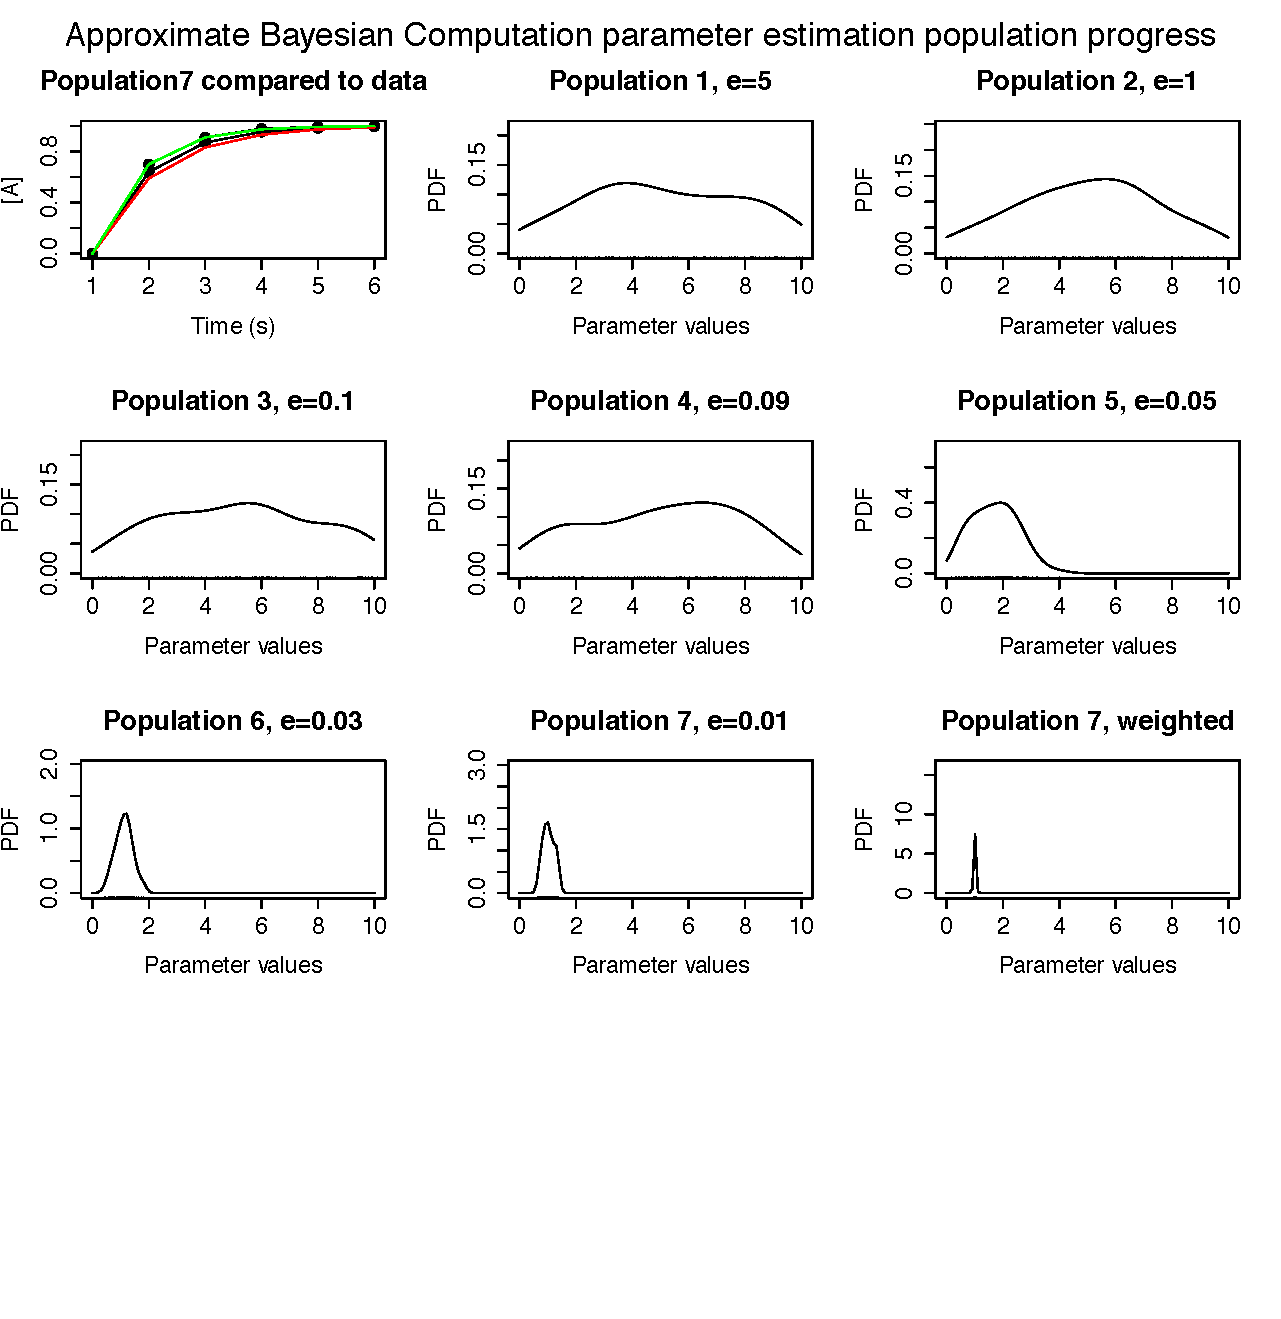
\includegraphics[scale=0.6]{../../chapters/chapterIntroduction/images/abcsmc_ex.pdf}
    \caption[\acrshort{abc} \acrshort{smc} parameter inference example]{ABC SMC parameter inference. The posterior parameter is equal to 1 and its time course shown in red in the top left panel. The blue time course is that of the final population, green is the upper quartile and red is the lower quartile range of values. The progress of the selection process can be seen the \textepsilon schedule proceeds from the top left to the bottom right. The bottom far right panel is a density plot of \textepsilon = 0.01 with their weights taken into account.  }
    \label{fig:myABC true 1}
    \end{center}
\end{figure*}
\clearpage

Figure~\ref{fig:myABC true 1} demonstrates, using a simple example, that \acrshort{abc} \acrshort{smc} is capable of fitting a model to the data. During the course of 7 populations, the accepted distance \textepsilon{} of the simulated particles to the data is incrementally decreased. This leads to a final population where the distance of the data to the particles is very small, and there is a good agreement between the two. The algorithm concludes with a set of parameter values that produced this behaviour, which approximate the posterior distribution. The posterior distribution found in this model is in good agreement with the parameter value used to generate the data. This example successfully demonstrates the effectiveness of the \acrshort{abc} \acrshort{smc} algorithm in fitting models to data. 

\subsection{Derivation of model parametric robustness defined via Bayesian statistics}
\label{sec:rob_back}
During this thesis I define robustness as the ability of a system to retain its function despite parameter perturbations~\autocite{Stelling:2004wo}. The robustness of biological systems has been studied extensively~\autocite{Barkai:1997cd, Stelling:2004wo, Prill:2005fq, Kim:2006uk, Kitano:2007cp, Hafner:2009ct, Shinar:2010dd, ZamoraSillero:2011jw, Woods:2016eh}. and it is well known that feedback loops can increase the robustness of a system~\autocite{Becskei:2000ft,	 DOYLE:2005ul}.

The robustness of a model can be calculated by dividing the volume of its functional region by the volume of its priors. This is a measure of the volume of the posterior distribution is compared to the priors. It comes from Bayes' rule that:

\begin{align}
	f(\theta|x) &= \frac{f(\theta)f(x|\theta)}{\int p(x|\theta)p(\theta)d\theta}
\end{align}

\noindent where $p(x|\theta)$ is the likelihood, $p(\theta)$ is the prior, and $\displaystyle \int p(x|\theta)p(\theta)d\theta$ is the evidence. The evidence is the normalisation  added so that the distribution integrates to 1. For a given model design D and objective O we define the functional region $F$ as the region within the prior where O is satisfied. So within the prior we can assign 1 to any region that falls within $F$ and 0 to any region outside that. 

\begin{align}
p(O|D_1) = \int p(O|\theta,D_1)p(\theta|D_1)d\theta,
\end{align}

\noindent For a design with three parameters this becomes:

\begin{align}
p(O|D_1) &= \displaystyle \iiint_{\underline{\Theta}} p(O|\underline{\Theta})p(\underline{\Theta}|D_1)d\underline{\Theta},
\end{align}

\noindent where $\underline{\Theta}$ is a vector containing the three parameters $ = \theta_1, \theta_2,\theta_3$. To calculate the robustness, or model evidence, we integrate this with respect to $\underline{\Theta}$. We assume  all parameters $\theta_1, \theta_2,\theta_3$ are uniform, $p(\underline{\Theta}|D_1) \sim U(a, b)$. If we assume a = 0 this integral becomes:

\begin{align}
p(O|D_1) &= \displaystyle \iiint_{\underline{\Theta}} p(O|\underline{\Theta})\frac{1}{b_1}\frac{1}{b_2}\frac{1}{b_3}d\underline{\Theta} \text{ , and }\\
p(O|D_1) &= \frac{1}{b_1}\frac{1}{b_2}\frac{1}{b_3} \displaystyle \iiint_{\underline{\Theta}}p(O|\underline{\Theta})d\underline{\Theta} \label{eq:1.6}
\end{align}

\noindent since $\frac{1}{b_1}\frac{1}{b_2}\frac{1}{b_3} $ is a constant. Then assuming that the likelihood is uniform Equation~\ref{eq:1.6} becomes:

\begin{align}
p(O|D_1) &= \frac{1}{b_1}\frac{1}{b_2}\frac{1}{b_3} \bigg[\displaystyle \iiint_{\underline{\Theta}_F} 1 d\underline{\Theta} +\cancelto{0}{\displaystyle \iiint_{\underline{\Theta}_{\cancel{F} }} 0 d\underline{\Theta}}\bigg]  \\
\end{align}
\noindent since we assign 1 to any region within $F$ and 0 to any region outside it. This becomes:
\begin{align}
p(O|D_1) &= \overbrace{\frac{1}{b_1}\frac{1}{b_2}\frac{1}{b_3}}^{|P|} \underbrace{\displaystyle \iiint_{\underline{\Theta}_F} 1 d\underline{\Theta}}_{|F|}, \\
\therefore p(O|D_1) &= \frac{|F|}{|P|},
\end{align}
where |P| is the volume of the prior P and |F| the volume of the functional region F. Therefore, in the case where both the prior and the likelihood are uniform, the robustness $R$ of the design is the ratio of the volumes of the two. If on the other hand we assume the likelihood is multivariate normal, with priors remaining uniform, Equation~\ref{eq:1.6} becomes: 
%normal
%\begin{align*}
%p(O|\underline{\Theta}) = c \times exp\bigg(-\frac{(O-\mu)^2}{2\sigma^2}\bigg)
%\end{align*}



%\begin{align}
%p(O|D_1) &= \frac{1}{|P|}\iiint_{\underline{\Theta}}f(\underline{\Theta};\mu,\Sigma)d\underline{\Theta} \\%, & \parbox[c]{\Sigma = \det(\text{covariance matrix})} \\
%\therefore p(O|D_1) &= \frac{1}{|P|}\underbrace{\times(2\pi)^\frac{k}{2}\times |\Sigma|^\frac{1}{2}}_{|F|} \\
%\therefore p(O|D_1) &= \frac{|F|}{|P|},
%\end{align}

\begin{align}
p(O|D_1) &= \frac{1}{|P|}\iiint_{\underline{\Theta}}f(\underline{\Theta};\mu,\Sigma)d\underline{\Theta} \\%, & \parbox[c]{\Sigma = \det(\text{covariance matrix})} \\
\therefore p(O|D_1) &= \frac{1}{|P|}\underbrace{\frac{2\pi^{\frac{k}{2}}}{k\Gamma(\frac{k}{2})} \Big[ \chi _{k}^{2}(\alpha) \Big]^{\frac{k}{2}} |\Sigma|^\frac{1}{2}} \\
\therefore p(O|D_1) &= \frac{|F|}{|P|},
\end{align}

%\begin{align}
%	V & = \frac{2\pi^{\frac{k}{2}}}{k\Gamma(\frac{k}{2})} \Big[ \chi _{k}^{2}(\alpha) \Big]^{\frac{k}{2}} |\Sigma|^\frac{1}{2}, \label{eq:el_vol}
%\end{align}


\noindent We can use the Bayes' factor in order to compare the robustness between two model designs. The Bayes' factor is defined as follows:

\begin{align}
B_{ab} &= \frac{\displaystyle \int p(x|\theta, D_a)p(\theta, D_a)d\theta}{\displaystyle \int p(x|\theta, D_b)p(\theta, D_b)d\theta} \\
\therefore B_{ab} &= \frac{|Fa|}{|Pa|} / \frac{|Fb|}{|Pb|} \label{eq:final_bayes}
\end{align}

\noindent Therefore, we can use the ratio of the two robustness measures to calculate the Bayes' factor. If two models have a different number of parameters, the robustness of the system will only increase if |F| increases by more than the proportion by which |P| increased~\autocite{Woods:2016eh}. A model will be penalised for an additional if it does not increase the volume of the functional region by more than the volume that the added parameter added to the prior. This is true for nested models, where one model is wholly contained in the other. 

%\section{Flow Cytometry}


%\section{Control theory in systems biology}

